%-------------------------
% CV in Chinese
% Author: Gavin OP
% Created time: 2021/04/01
% Enquiry: 564493609@qq.com
% This work can be modified under latex
% Copyright. All rights reserved.
%-------------------------

% Paper size
\documentclass[a4paper]{article}

% Declare packages
\usepackage[UTF8]{ctex}
\usepackage[margin=1in]{geometry}
\usepackage[hidelinks]{hyperref}
\usepackage{titlesec}
\usepackage{enumitem}
\usepackage[usenames,dvipsnames]{color}
\usepackage{tabularx}
\usepackage{fancyhdr}
\usepackage{graphicx}


% Adjust margins
\geometry{textheight=20cm}
\geometry{left=1cm}
\geometry{right=1cm}
\geometry{top=0.7cm}
\geometry{bottom=1cm}

% Sections formatting
\titleformat{\section}{
  \vspace{-6pt}\heiti\raggedright\large
}{}{0em}{}[\color{black}\titlerule \vspace{-4pt}]

% Set link color
\hypersetup{colorlinks=true, urlcolor=blue}

% Clear all header and footer fields
\pagestyle{fancy}
\fancyhf{} % Clear all header and footer fields
\fancyfoot{}
\renewcommand{\headrulewidth}{0pt}
\renewcommand{\footrulewidth}{0pt}



% Custom commands
\newcommand{\resumeItem}[1]{
    \item\small{
        {#1 \vspace{-3pt}}
    }
}


\newcommand{\resumeSubOPheading}[5]{
    \vspace{-3pt}\item\renewcommand\arraystretch{0.8}
    \begin{tabular*}{0.99\textwidth}[t]{l@{\extracolsep{\fill}}r}
        \heiti{\small#1} & \small#2 \\
        \textit\heiti{\small#3} & \textit\heiti{\small #4} \\
        \textit\heiti{\small#5} \\
    \end{tabular*}\vspace{-8pt}
}

\newcommand{\resumeSubheading}[4]{
    \vspace{-3pt}\item\renewcommand\arraystretch{0.8}
    \begin{tabular*}{0.99\textwidth}[t]{l@{\extracolsep{\fill}}r}
        \heiti{\small#1} & \small#2 \\
        \textit\heiti{\small#3} & \textit\heiti{\small #4} \\
    \end{tabular*}\vspace{-7pt}
}





\newcommand{\resumeSubHeadingListStart}{\begin{itemize}[leftmargin=0.15in, label={}]}
\newcommand{\resumeSubHeadingListEnd}{\end{itemize}}
\newcommand{\resumeItemListStart}{\begin{itemize}}
\newcommand{\resumeItemListEnd}{\end{itemize}\vspace{-6pt}}

\renewcommand\labelitemii{$\vcenter{\hbox{\tiny$\bullet$}}$}








\begin{document}

\begin{center}
    \heiti{\LARGE 张皓翔} \\ \vspace{1pt}
    \small +86 15099684758 $|$
    \href{mailto:HaoxiangZhang@link.cuhk.edu.hk}{{HaoxiangZhang@link.cuhk.edu.hk}} $|$
    \href{https://linkedin.com/in/gavin-zhang-op}{{linkedin.com/in/gavin-zhang-op}} 
\end{center}

\begin{picture}(1,1)
\put(462,2){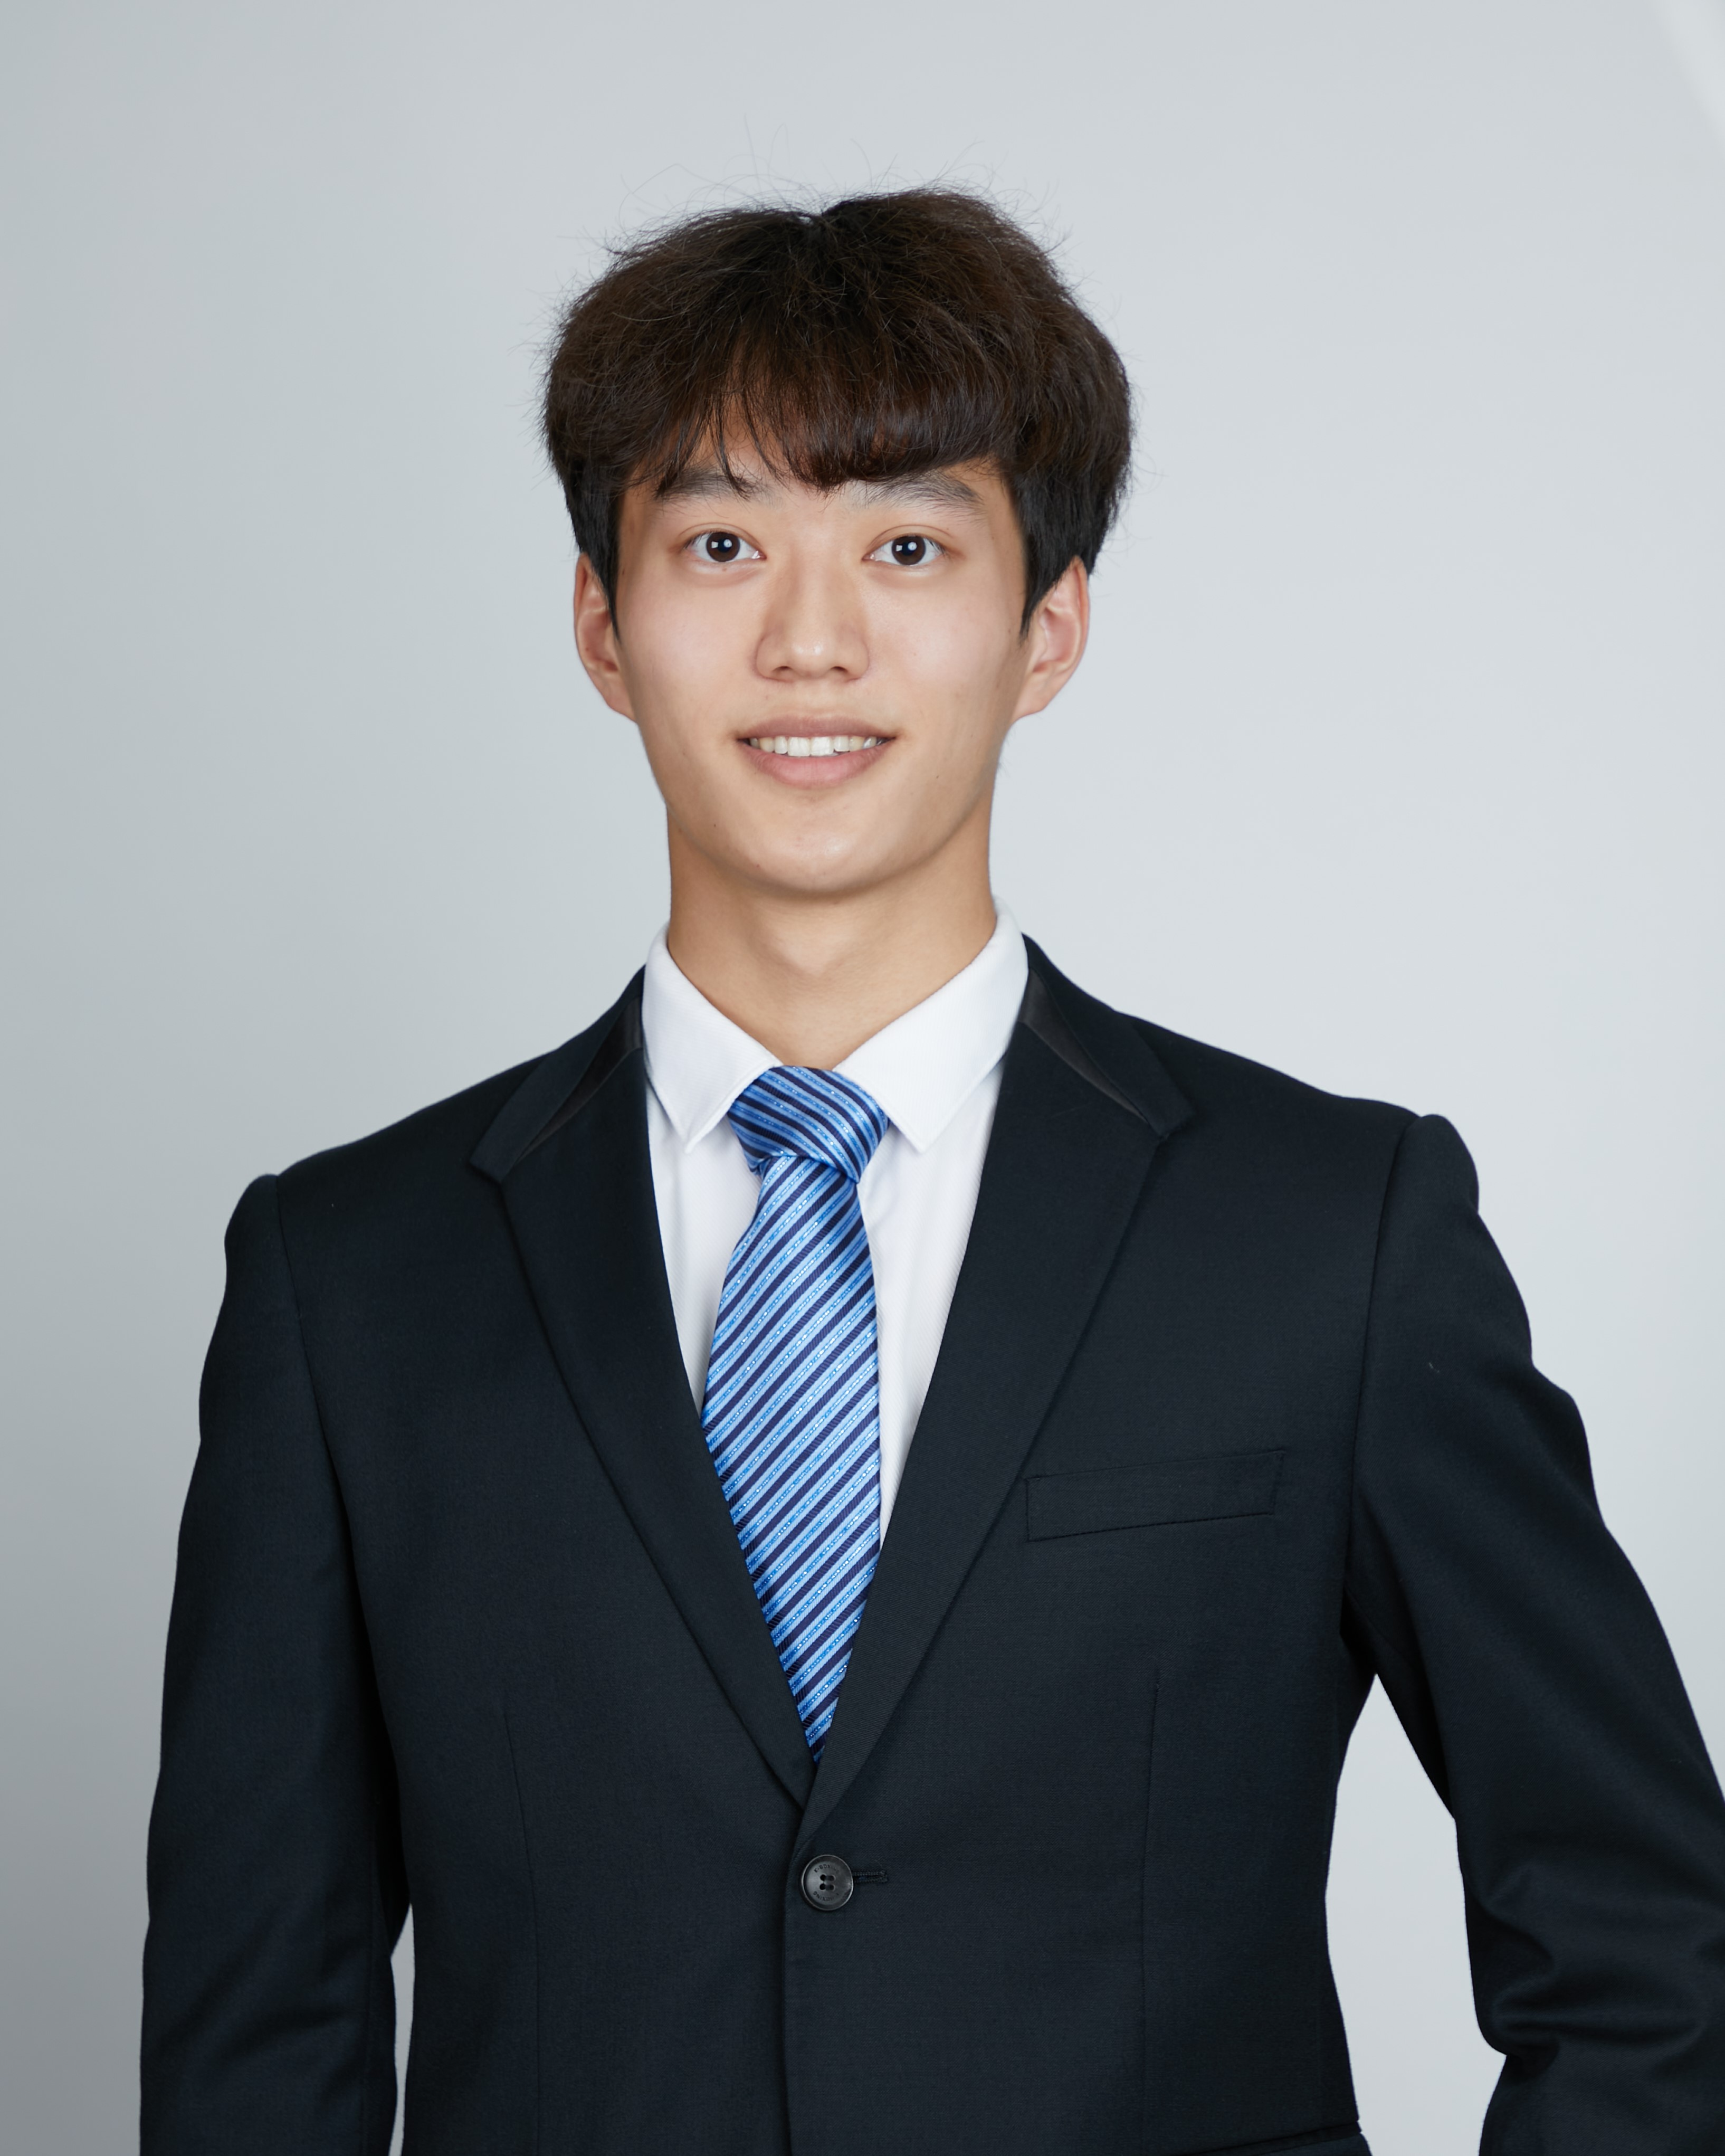
\includegraphics[width=0.75in]{1.png}}
\end{picture}\vspace{-36pt}


%-----------自我评价-----------
\section{自我评价}
    \begin{itemize}[leftmargin=0.15in, label={}]
        \small{\item{一个勤奋的CHUK学生,在南洋理工大学和Coursera学习额外课程,同时管理五个协会和组织志愿者团队。为大流行期间的俱乐部活动建立在线模式,服务新岗位,以适应团队的变化。}}
    \end{itemize}\vspace{-17pt}



%-----------教育背景-----------
\section{教育背景}
    \resumeSubHeadingListStart
        \resumeSubOPheading
            {香港中文大学\textbf{(CUHK)}}{香港,新界}
            {本科;计量金融与风险管理;cGPA:3.680/4 (Dean’s list) }{2019.09 -- 至今}
            {奖项:2019/20人才发展奖学金, 2020/21郑栋材奖学金,UBC校友会奖学金}
        \resumeSubheading
            {南洋理工大学\textbf{(NTU)}}{新加坡}
            {APRU线上交换项目:海上丝绸之路。继承和媒体}{2021.01 -- 2021.05}
        \resumeSubheading
            {乌鲁木齐市第一中学}{中国,新疆}
            {高考成绩: 643/750;排名:理科第243名}{2019.06}
  \resumeSubHeadingListEnd



\section{工作经历}
    \resumeSubHeadingListStart
        \resumeSubheading
            {普华永道}{中国,北京}
            {审计暑期实习生 $|$ 亚洲基础设施投资银行\textbf{(AIIB)}项目组}{2021.07 -- 2021.08}
        \resumeItemListStart
            \resumeItem{汇总由AIIB发行的20+国家,75支主权贷款的Moody’s、S\&P、Fitch信用评级,并将其与历史评级、AIIB评级报告、AIIB会议纪要等文件比较,为内部评级复核提供数据支持。}
            \resumeItem{核对ESG债券的投资交易记录与试算平衡表,保证业务账与财务账的一致性;抽样核查ESG债券利息收入和摊销额,保证债券利息收入以及余额的准确性。}
            \resumeItem{根据S\&P测试程序使用手册标准,评估2个亚投行非主权贷款金融项目评级测试程序,审核其与项目文件、项目进度报告、项目实施监测报告等文件的一致性,并客观反馈评级准确性。}
            \resumeItem{根据同事有关历史价格、信用评级、交易记录、运营趋势等方面的需求,使用彭博终端检索有效数据并加以总结,为后续审计工作提供数据。}
            \resumeItem{对财政、其他综合收入、贷款进行控制测试,审核各控制点的一致性、交易证据的连续性、测试程序的完整性。}
        \resumeItemListEnd
    
    
        \resumeSubheading
            {知乎}{中国,北京}
            {商务拓展实习生 $|$ 视频融合及内容运营}{2021.04 -- 2021.07}
        \resumeItemListStart
            \resumeItem{审核4个外包公司提报的3000+个博主账号,根据创作者分类标准划分账号等级及领域。引导1200+位高质博主参与扶持计划,入驻知乎社区,并激励他们保持创作活跃度,发布符合当前热点的高质视频。}
            \resumeItem{使用SQL从知乎数据库中检索视频运营数据,使用R语言设计并编写视频拓展状态周报表。处理并监控数据以预测未来发展,从而合理调整扶植计划,最小化预算。}
            \resumeItem{下发800+份电子协议并统计签署情况。为高质热门视频分配首页槽位流量。适用网页端口协助社区运营、账号授权、批量下架视频、更改发布上限等。}
        \resumeItemListEnd
    \resumeSubHeadingListEnd



\section{社团经历}
    \resumeSubHeadingListStart

        \resumeSubheading
            {香港新疆联谊会}{香港,新界}
            {秘书处成员}{2019秋 -- 至今}
        \resumeItemListStart
            \resumeItem{代表联谊会收集60+名赴港新疆新生信息,联络后提供生活、学术等方面的帮助,协助主席团安排迎新日,参与人数50+人。}
            \resumeItem{协助主席团组织2021太平杯·互融青年慈善篮球联赛,与参与者沟通后敲定训练细则,帮助会员拓展社交圈,促进会员关系。}
        \resumeItemListEnd
      

        \resumeSubheading
            {香港中文大学联合书院学生会内地本科生联合会}{香港,新界}
            {会长}{2020.03 -- 2021.03}
        \resumeItemListStart
            \resumeItem{协调11名联合会成员组织2次分享会、1次迎新日、1次交职典礼、1次疫情期间毕业生行李转运、以及多项娱乐活动,并通过邮件,微信公众号,微信小程序等方式进行前期宣传和后期总结,共发送70+篇微信公众号推送。}
            \resumeItem{编写联合会年度计划,主持30+次例会,设计社团线上竞选机制,引领联合会帮助约250名会员适应大学生活,融入香港文化。}
            \resumeItem{代表内地本科生与联合书院谈判,经过多次沟通协商后,维护了内地本科生合理住宿权益,保留并顺延宿位直至面授开始。}
        \resumeItemListEnd


        \resumeSubheading
            {三心社}{香港,新界}
            {大组长}{2020.12}
        \resumeItemListStart
            \resumeItem{设计并制作了8节义教课程,用幽默风趣的方式帮助河南贫困高中的10名同学掌握反冲,统计等问题,授课时长10+小时。}
            \resumeItem{带领义教团确定主题,设计流程,举行了1次拓展活动及1次高考经验分享会,为100+高中生介绍大学生活及学习方法。}
        \resumeItemListEnd


        \resumeSubheading
            {扶葭}{香港,新界}
            {人力资源}{2019秋 -- 2020秋}
        \resumeItemListStart
            \resumeItem{协助团队成员分工撰写深圳荔枝项目组策划书,主持月度例会,安排团建活动,制作招新宣传视频及推广推送。}
            \resumeItem{设计面试流程和题目,撰写招募标准等相关文件,招募志愿者并组织破冰活动及培训,带领志愿者对30+名深圳留守儿童进行了为期8小时的知识传授、生活辅导等。}
        \resumeItemListEnd
      
      
        \resumeSubheading
            {乌鲁木齐市一中健美操队}{中国,新疆}
            {队长}{2016.09 -- 2019.06}
        \resumeItemListStart
            \resumeItem{管理健美操队的日常训练,设计参赛舞蹈动作,代表乌鲁木齐市一中获得2次全国啦啦冠军赛第一名及众多其他奖项。}
        \resumeItemListEnd

  \resumeSubHeadingListEnd



\section{其他经历}
    \resumeSubHeadingListStart
        \resumeSubheading
            {情系博达微信公众平台}{中国,新疆}
            {负责人}{2019秋 -- 现在}
        \resumeItemListStart
            \resumeItem{发起并邀请来自28所高校的校友录制2020年高考加油视频并发布于B站和微信公众号,转载于乌鲁木齐市一中官方公众号及校园电子班牌,累计浏览量约为16000次,在高考前为高三考生加油鼓劲。}
            \resumeItem{策划并组织了43场线上校友直播宣讲会,共邀请38所大学100+校友参与宣讲,与《晨报》达成后期合作,宣讲会累计观看量超过10000人,并动员校友投稿,发送35+篇介绍大学及专业的推送。}
         \resumeItemListEnd
    
    
        \resumeSubheading
        {\textbf{CUHK i-ambassador}}{香港,新界}
         {负责人}{2019.08 -- 2021.02}
        \resumeItemListStart
            \resumeItem{带领团队查阅新疆文化资料并从多角度分析总结,最终通过线上工作坊的方式介绍新疆的饮食、地理、风俗、节日等,邀请多名来自不同国家和地区的学生了解新疆文化。}
        \resumeItemListEnd
    
    
        \resumeSubheading
            {香港中文大学2020内地本科生迎新营}{香港,新界}
            {志愿者}{2020秋}
        \resumeItemListStart
            \resumeItem{总结大学衣食住行攻略,开展工作坊介绍校园生活、设施、香港文化等,帮助新生快速适应大学生活,为期5天。}
        \resumeItemListEnd
    
    
        \resumeSubheading
            {香港中文大学普通话剧社}{香港,新界}
            {演员}{2019秋 -- 202.01}
        \resumeItemListStart
            \resumeItem{在秋戏《庄先生》中饰演楚王孙和楚天,经过两个月的训练与排练,于逸夫书院大讲堂演出2次,累计观众100+人。}
        \resumeItemListEnd
        
        
        \resumeSubheading
            {香港中文大学2019内地本科生迎新晚会}{香港,新界}
            {主持人}{2019秋}
        \resumeItemListStart
            \resumeItem{策划晚会流程,撰写主持文案,组织并主持迎新晚会,使节目顺利进行,共有观众500+人。}
        \resumeItemListEnd
        
        
    \resumeSubHeadingListEnd



\section{技能和兴趣}
    \begin{itemize}[leftmargin=0.15in, label={}]
        \small{\item{
            \heiti{编程:}{基础:C++,R,SAS,Python,LaTex,SQL,Markdown,Pr,Bloomberg;熟练:PowerPoint,Excel;精通:微信公众号} \\
            \heiti{语言:}{普通话(母语),英语(流利,托福:104/120),粤语(基础)}\\
            \heiti{兴趣:}{山地车,游泳,登山,健美操,手风琴,制作vlog,数独} 
        }}
    \end{itemize}




\end{document}
